% chapter16.tex -- Future Work
% Based on the author's UGThesis.docx.

\chapter{Future Work}
\label{ch:future_work}

In this chapter we outline several directions for extending the results of this thesis. 
The most immediate open problem is the extension of our algorithm to 1-connected plane graphs, which faces fundamental obstacles as discussed in Chapter~\ref{ch:one_connected}. 
Other promising directions include the generation of triangulations for 1-planar graphs, parallelisation, and canonical representations for unlabeled triangulations.

\section{Extension to 1-Connected Graphs}
\label{sec:future_1connected}

As shown in Chapter~\ref{ch:one_connected}, our algorithm cannot be applied directly to all 1-connected plane graphs because faces may contain a vertex multiple times, and a safe root may not exist. 
Nevertheless, we have identified a subclass of 1-connected graphs where a safe root does exist (e.g., the graph of Figure~\ref{fig:lollipop}). 
A possible direction is to characterise exactly which 1-connected graphs admit a safe root in every face, and to modify the algorithm to handle those that do not.

One approach is to preprocess the graph by splitting at cut vertices, decomposing it into biconnected components. 
Each biconnected component can be triangulated independently using our algorithm, and then the triangulations can be combined. 
However, the combination step must ensure that chords do not conflict across components, which is non-trivial because cut vertices are shared. 
This is reminiscent of the SPQR tree decomposition for planar graphs, and we believe that a recursive decomposition could lead to an algorithm for all 1-connected plane graphs, possibly with the same optimal complexity.

Another direction is to allow a controlled amount of multi-edges during generation, and then remove them in a post-processing step. 
But this would likely violate the \(O(1)\) amortised time guarantee.

\section{Extension to 1-Planar Graphs}
\label{sec:future_1planar}

A graph is \textbf{1-planar} if it can be drawn in the plane such that each edge is crossed at most once. 
1-planar graphs are a well-studied generalisation of planar graphs and have applications in graph drawing and network visualisation. 
Generating all triangulations of 1-planar graphs (maximal 1-planar graphs) is an open problem.

Our algorithm for biconnected plane graphs relies heavily on planarity: chords cannot cross, and the flipping operation preserves planarity. 
In a 1-planar drawing, edges may cross, but at most one crossing per edge pair. 
A triangulation of a 1-planar graph is a maximal set of edges such that each face is a triangle, but crossings are allowed. 
The notion of a “flip” becomes more complex because flipping a chord might increase or decrease the number of crossings.

\begin{figure}[htbp]
    \centering
    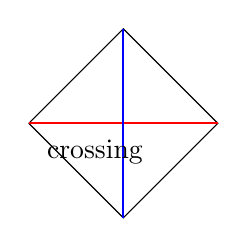
\begin{tikzpicture}[scale=1.2]
        % A simple 1-planar graph: K5 drawn with one crossing
        \coordinate (A) at (0,1);
        \coordinate (B) at (1,0);
        \coordinate (C) at (2,1);
        \coordinate (D) at (1,2);
        \coordinate (E) at (1,1);
        \draw (A)--(B)--(C)--(D)--(A);
        \draw (A)--(C);
        \draw (B)--(D);
        \draw (E)--(A);
        \draw (E)--(B);
        \draw (E)--(C);
        \draw (E)--(D);
        \draw[red, thick] (A)--(C);
        \draw[blue, thick] (B)--(D);
        \node at (0.7,0.7) {crossing};
    \end{tikzpicture}
    \caption{A 1-planar graph (the complete graph \(K_5\) drawn with one crossing). 
    Edge flips may change the crossing pattern.}
    \label{fig:one_planar}
\end{figure}

Nevertheless, the genealogical tree approach might be adaptable: we could define a parent-child relationship based on flipping an edge that does not increase the number of crossings, or that reduces a suitable potential function. 
The safe root concept would need to be redefined because chords may cross existing chords. 
We believe that our technique of processing faces sequentially and pruning invalid branches could be extended to 1-planar graphs, but substantial new theory is required.

\section{Parallel Generation of Triangulations}
\label{sec:parallel}

The genealogical tree is inherently a recursive structure, but it is not balanced. 
However, the root triangulation has many children, and subtrees are independent. 
This suggests that the generation process could be parallelised: different branches of the tree could be explored by different threads or processes.

A simple approach is to generate the first few levels of the tree sequentially, and then distribute the subtrees to worker threads. 
Because the tree has exponential size, even a coarse-grained parallelisation could yield significant speedups. 
We leave the design and analysis of a parallel version as future work.

\section{Canonical Representation for Unlabeled Biconnected Triangulations}
\label{sec:canonical}

Our algorithm works for labeled graphs (all vertices have distinct labels). 
For unlabeled graphs, we would need to avoid isomorphic triangulations (rotation and reflection symmetries). 
Parvez et al.~\cite{parvez2011} gave a method to generate unlabeled triangulations of a cycle by using the degree sequence as a canonical representation and pruning rotationally or reflectively equivalent triangulations. 
Extending this to biconnected plane graphs is more challenging because the graph may have non-trivial automorphisms.

One possible approach is to compute a canonical labelling of the input graph (e.g., using a planar graph isomorphism algorithm) and then only output triangulations that are canonical with respect to that labelling. 
Alternatively, we could modify the DFS to only explore triangulations that are lexicographically smallest under a suitable ordering. 
This is a promising direction for future research.

\section{Other Generalisations}
\label{sec:other_generalisations}

Our algorithm may also be adapted to generate all triangulations of:
\begin{itemize}
    \item Graphs on surfaces of higher genus (toroidal graphs, etc.), where the notion of “face” is still defined but the Euler characteristic changes.
    \item Graphs with pre-specified edges that must be included (constrained triangulations).
    \item Triangulations that respect a given outer face (fixed boundary).
\end{itemize}
Each of these directions requires careful modification of the safe root concept and the pruning strategy.

\section{Summary}
\label{sec:future_summary}

We have outlined several avenues for extending this work: handling 1-connected graphs via biconnected decomposition, generalising to 1-planar graphs, parallel generation, canonical output for unlabeled graphs, and other variants. 
The most immediate and challenging is the extension to 1-connected graphs, which would require a fundamental rethinking of face triangulation in the presence of cut vertices. 
We hope that the techniques developed in this thesis—safe root selection, persistent chord pruning, and multi-layer DFS—will serve as a foundation for these future investigations.